% $Rev: 811 $
% $LastChangedDate: 2011-08-10 10:05:04 +0200 (Mi, 10 Aug 2011) $ 
% $Author: meesters $ 
\chapter{Utilities}

This chapter attempts to describe all utilities easing your work with \textsc{yamas}. Note, that this documentation might not describe all you as a user might need to know: Just inform the \textsc{yamas}-developers about any additional information you require. Also, please inform us if you would like to provide a script which eases the work with \textsc{yamas} or would like to write us additional utility scripts.

All \textsc{yamas} Python scripts have a shebang and a \verb+__future__+-statement:
\begin{lstlisting}[style=Python]
#! /usr/bin/env python
from __future__ import with_statement
\end{lstlisting}
The shebang (\verb+#! ...+) lets unixoid operating systems find a script in the local \verb+PATH+, if made executable. The \verb+__future__+-statement limits the compatibility to $2.6 \leq \mathsf{Python-version} < 3$.


\section{Forest Plots}

A forest plot (sometimes called a ``blobbogram'') is a plot designed to illustrate the relative strength of effects in multiple quantitative scientific studies addressing the same question. In the case of GWAS-meta analyses a forest plot can be used to display the meta analysis result of a particular marker. Along with a \textsc{yamas} download a script which can produce a forest plot for a particular marker. The script is written in Python (\url{www.python.org}) and requires numpy \citep{Oliphant2007} and matplotlib \citep{Hunter2007}. Note that Python scripts are not compiled and require a Python interpreter in addition to the mentioned packages. Please consult your packaging system or download the interpreter from \url(www.python.org). 

Figure \ref{utilities:fig:forest_plot} on the following page shows a typical forest plot generated by the \verb+forest_plot+. The script is invoked like (UNIX or cygwin shell):
\begin{lstlisting}[style=shell]
$ <path>/forest_plot --configfile <configuration file> \
                     --result <result or logfile> \
                     --rsid <marker id of the marker to be extracted>
                     --xlabel [label of the x-axis]
\end{lstlisting}         
The command can be typed on one line, the \verb+\+ omitted. The configuration file and the result file are the respective files for the analysis you as the \textsc{yamas}-user have performed.

In addition the \verb+--dpi+-option lets you specify the resolution of the plot and the \verb+--extension+ the kind of the plot. Valid extensions are \verb+png+, \verb+ps+, and \verb+eps+. Additional kinds may be available, depending on your matplotlib installation. Please consult the matplotlib manual.

The \verb+--xlabel+-options lets you specify the label of the x-axis. \LaTeX expressions are valid, e.\,g. \verb+--xlabel "$\\beta_i$"+. Note however, that backslashes have to be escaped. This is why we see the two \verb+\\+ in the example.

\clearpage
\pagebreak

\begin{figure}[H]
 \centering
 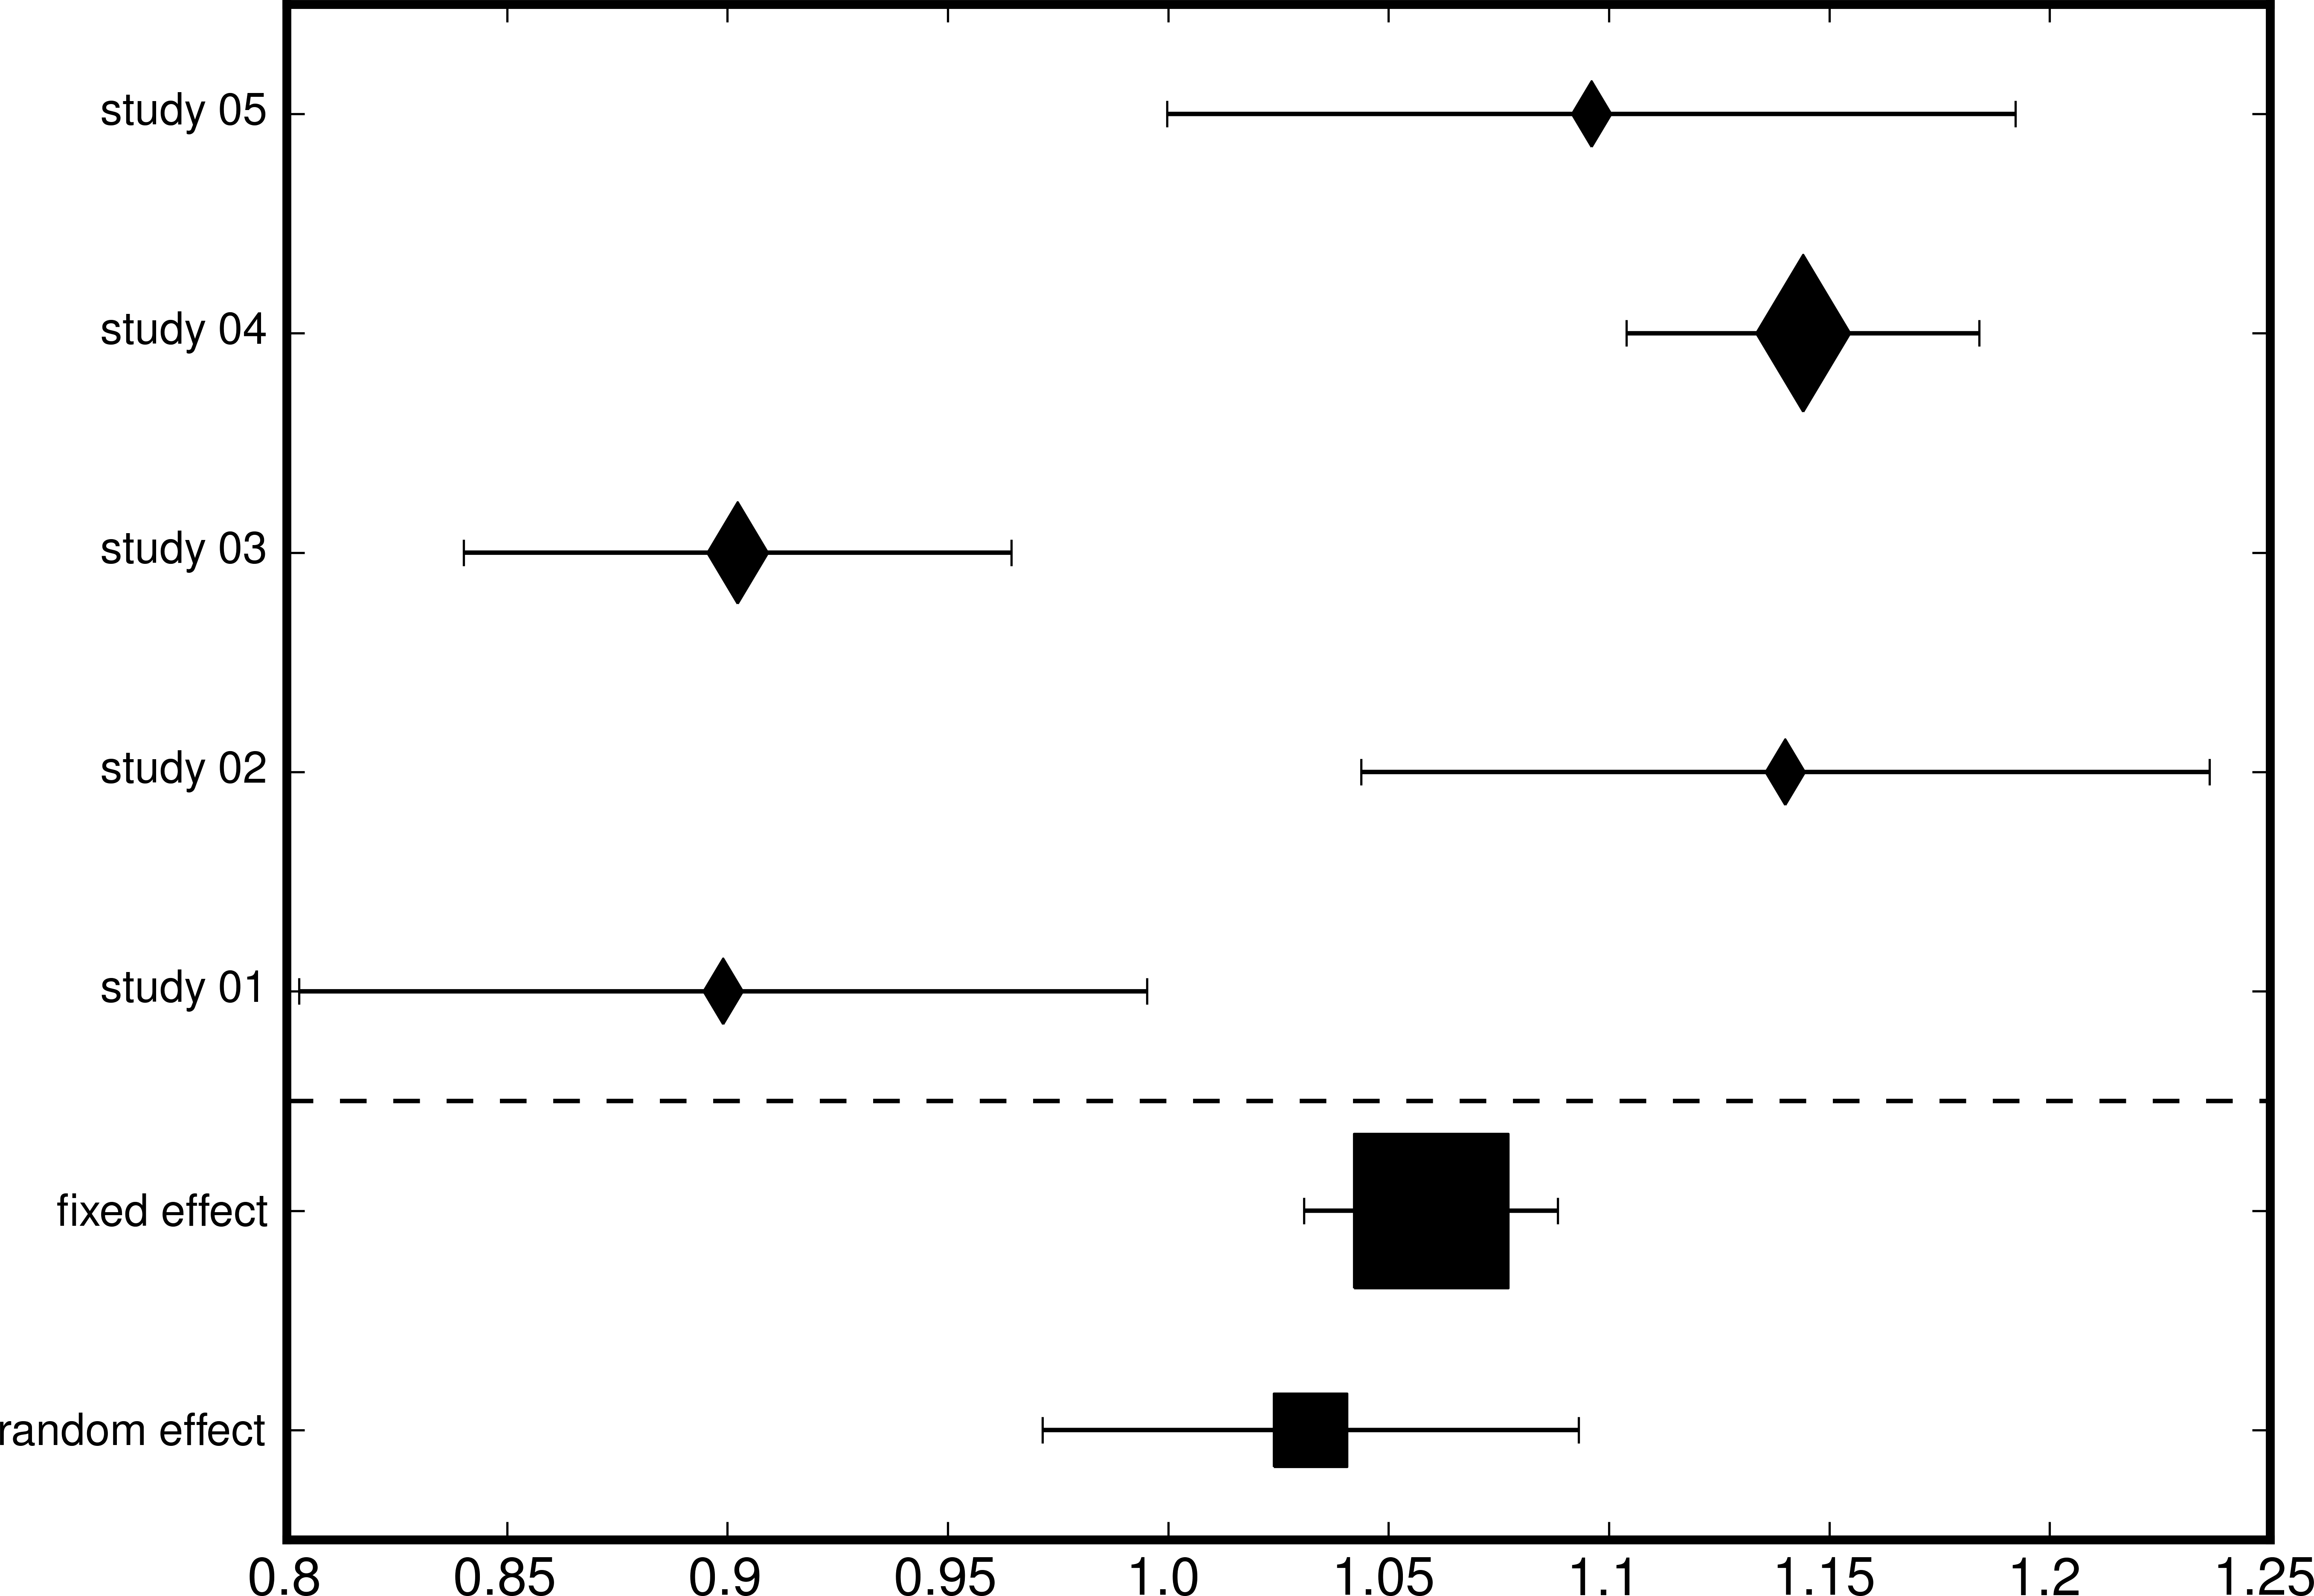
\includegraphics[width=.75\textwidth]{./images/rs9442372.png}
 \caption{Example forest plot for one particular marker showing how the more conservative random effect reflects the variance between studies. Note that the marker size (marker of the plot, not the GWAS) is inverse proportional to the standard error of that marker within a study or the meta-analysis.}
 \label{utilities:fig:forest_plot}
\end{figure}

\section{Switching Genotypes}

Occasionally studies may differ in there designation of effect and reference or other alleles for many markers. In this case \textsc{yamas} will refuse to consider these markers as valid, because the meta-analysis requires reliable effect directions and automatic corrections (described in paragraph \ref{algo:alleles}) cannot be accomplished if the genotypes aren't the same.

In this case the \verb+swith_markers+-script can change the genotypes of particular markers according to a reference. The script is invoked like

\begin{lstlisting}[style=shell]
$ <path>/switch_markers --configfile    <configuration file> \
                        --referencefile <the study file which \
                       genotypes should serve as a reference> \
                        --wrongfile     <the study file which \
                       genotypes should be corrected>
\end{lstlisting}

The command can be typed on one line, the \verb+\+ omitted.

Currently (as of \textsc{yamas} version 0.5) two cases are considered:
\begin{itemize}
 \item The genotypes are identical - hence, the genotypes in \verb+wrongfile+ are left untouched.
 \item The genotypes are each others complements - here, the genotypes in \verb+wrongfile+ for the respective marker are changed to their complements.
\end{itemize}

\section{Transforming \texttt{.vcf}-Files to Plink Compatible Format}

While \textsc{yamas} provides refrence files for the ``proxy-algorithm'' (see paragraph \ref{algo:fillwithproxies}, own reference files can be generated (see paragraph \ref{algo:own_refernce_files}). For this purpose Plink \citep{Purcell2007} compatible files are needed. Some projects, e.\,g. the 1000 genomes project, provide their data in the \texttt{vcf}-format. To transform \texttt{.vcf}-files into Plink \texttt{tped/tfam} file tuples, please have a look at the \texttt{vcf2tped} script in the utility directory of your download.  

\section{More Utilities?}

Obviously we cannot provide solutions for all imaginable problems which may come with meta-analysis. If you encounter a so far unsolved problem, please contact us: Either provide a general solution for that problem as a script (not necessarily Python) -- your name will be mentioned! -- or ask us for help, such that we can provide a script to solve your problem (in more complex cases we might ask for co-authorship).


